%!TEX root = supplemental.tex

TODO

- add additional cables results 

- add arxiv figure (see we dont find events!)

- add simulations for shape and duration


%%%%%%%%%%%%%%%%%%%

\parhead{}
contains additional examples of results for the 
Apollo 17 lunar gifts, the return of the crown of St. Stephen to Hungary, and the UN Special Session on Disarmament in 1978.


Another peak occurs the week of April 17, 1978 surrounding a UN special session on disarmament; the top three words under event its description $\pi$ are \emph{SSOD} (acronym for ``special session on disarmament'', \emph{disarmament}, and \emph{ICS} (likely an acronym for ``incident command system'').

more details on air france hijackign?

- more general end entity specific topics

Capsule also identifies smaller events, including the International Whaling commission (IWC) ban on killing bowhead whales in early October of 1977.  The top cables recovered by Capsule indicate that the U.S. State department objected to this ban because Alaskan Natives rely on these whales for sustenance.

Another sequence of events occurs surrounding opium production; in March 1974, Capsule detects that Turkey plans to lift a ban on growing opium poppy.  Two months later, the model detects another event when the U.S. makes a policy statement on the domestic production of opium poppy.


\parhead{arXiv event detection.}

\begin{figure*}[ht]
\centering
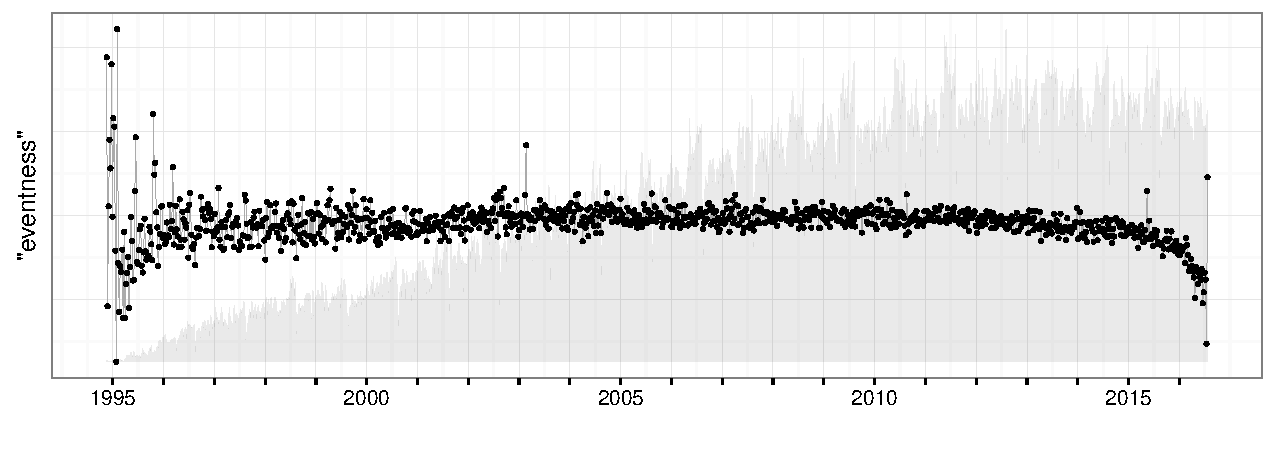
\includegraphics[width=\linewidth]{fig/arxiv_events.pdf}
\caption{Measure of time interval impact on cable content (Eq.~\ref{eq:eventness}).  Grey background indicates the number of abstracts submitted over time.}
\label{fig:arxiv_events}
\end{figure*}